%% This is the ctufit-thesis example file. It is used to produce theses
%% for submission to Czech Technical University, Faculty of Information Technology.
%%
%% Get the newest version from
%% https://gitlab.fit.cvut.cz/theses-templates/FITthesis-LaTeX

% arara: xelatex
% arara: biber
% arara: xelatex
% arara: xelatex

%%%%%%%%%%%%%%%%%%%%%%%%%%%%%%%%%%%%%%%%%
% CLASS OPTIONS
% language: czech/english/slovak
% thesis type: bachelor/master/dissertation
% colour: bw for black&white OR no option for default colour scheme
% electronic (oneside) or printed (twoside), twoside is default
% paragraph - if passed, this optional argument sets paragraphs as the deepest level of headers, styles it, numbers it and adds it to Table of Content. Use with care! Normally, it is considered unwise to use it, since its too deep.
%%%%%%%%%%%%%%%%%%%%%%%%%%%%%%%%%%%%%%%%%
\documentclass[english,bachelor,bw,unicode,twoside]{ctufit-thesis}

%%%%%%%%%%%%%%%%%%%%%%%%%%%%%%%%%%
% FILL IN THIS INFORMATION
%%%%%%%%%%%%%%%%%%%%%%%%%%%%%%%%%%
\ctufitauthorsurnames{Laštovička}
\ctufittitle{NAC-colorings search: complexity and algorithms}
\ctufitauthorfull{Petr Laštovička}
\ctufitauthorgivennames{Petr}
\ctufitsupervisor{Dr.\,techn.\,Ing.\,Jan Legerský}
\ctufitdepartment{Faculty of Theoretical Informatics}
\ctufityear{2025}
\ctufitdeclarationplace{Prague}
\ctufitdeclarationdate{\today} % replace with the date of signature of the declaration
\ctufitabstractCZE{Fill in the abstract of this thesis in Czech. Lorem ipsum dolor sit amet. Class aptent taciti sociosqu ad litora torquent per conubia nostra, per inceptos hymenaeos. Cras pede libero, dapibus nec, pretium sit amet, tempor quis. Sed vel lectus. Donec odio tempus molestie, porttitor ut, iaculis quis, sem. Suspendisse sagittis ultrices augue.}
\ctufitabstractENG{Fill in the abstract of this thesis in English. Lorem ipsum dolor sit amet. Class aptent taciti sociosqu ad litora torquent per conubia nostra, per inceptos hymenaeos. Cras pede libero, dapibus nec, pretium sit amet, tempor quis. Sed vel lectus. Donec odio tempus molestie, porttitor ut, iaculis quis, sem. Suspendisse sagittis ultrices augue.}
\ctufitkeywordsCZE{enter, comma, separated, list, of, keywords, in, CZECH}
\ctufitkeywordsENG{enter, comma, separated, list, of, keywords, in, ENGLISH}
%%%%%%%%%%%%%%%%%%%%%%%%%%%%%%%%%%
% END FILL IN
%%%%%%%%%%%%%%%%%%%%%%%%%%%%%%%%%%

%%%%%%%%%%%%%%%%%%%%%%%%%%%%%%%%%%
% CUSTOMIZATION of this template
% Skip this part or alter it if you know what you are doing.
%%%%%%%%%%%%%%%%%%%%%%%%%%%%%%%%%%

\RequirePackage{iftex}[2020/03/06]
\iftutex{}% XeLaTeX and LuaLaTeX
    \RequirePackage{ellipsis}[2020/05/22] %ellipsis workaround for XeLaTeX
\else
    \errmessage{Only compilation with XeLaTeX or LuaLaTeX is allowed}
    \stop
\fi

% hyperlinks
\hypersetup{
    pdfpagelayout=TwoPageRight,
    colorlinks=false,
    allcolors=decoration,
    pdfborder={0 0 0.1}
}

% uncomment the following to hide all hyperlinks
%\hypersetup{hidelinks}

% uncomment the following to change the color of all hyperlinks to CTU blue
\hypersetup{allbordercolors=decoration}

\RequirePackage{pdfpages}[2020/01/28]

%%%%%%%%%%%%%%%%%%%%%%%%%%%%%%%%%%
% CUSTOMIZATION of this template END
%%%%%%%%%%%%%%%%%%%%%%%%%%%%%%%%%%


%%%%%%%%%%%%%%%%%%%%%%
% CONTENTS SETTINGS
%%%%%%%%%%%%%%%%%%%%%%
\usepackage{dirtree}
\usepackage{lipsum,tikz}
\usepackage[style=iso-numeric]{biblatex}
\addbibresource{text/bib-database.bib}
\usepackage{xurl}
\usepackage{listings} % typesetting of sources
%\usepackage{minted}
\usepackage{csquotes}

%%%%%%%%%%%%%%%%%%%%%%
% CONTENTS SETTINGS END
%%%%%%%%%%%%%%%%%%%%%%

%%%%%%%%%%%%%%%%%
% CUSTOM COMMANDS
%%%%%%%%%%%%%%%%%
\newcommand{\MSO}{\(\text{MSO2}\)}
%%%%%%%%%%%%%%%%%
% CUSTOM COMMANDS END
%%%%%%%%%%%%%%%%%


\begin{document}
\frontmatter\frontmatterinit{} % do not remove these two commands

\thispagestyle{empty}\maketitle\thispagestyle{empty}\cleardoublepage{} % do not remove these four commands

\includepdf[pages={1-}]{./assignment.pdf} % thesis assignment generated from ProjectsFIT

\imprintpage{} % do not remove this command
\stopTOCentri
%%%%%%%%%%%%%%%%%%%%%%
% list of other contents END
%%%%%%%%%%%%%%%%%%%%%%

%%%%%%%%%%%%%%%%%%%
% ACKNOWLEDGMENT
% This is a place to thank people for helping you. It is common to thank your supervisor.
%%%%%%%%%%%%%%%%%%%
\begin{acknowledgmentpage}
	Chtěl bych poděkovat především sit amet, consectetuer adipiscing elit. Curabitur sagittis hendrerit ante. Class aptent taciti sociosqu ad litora torquent per conubia nostra, per inceptos hymenaeos. Cras pede libero, dapibus nec, pretium sit amet, tempor quis. Sed vel lectus. Donec odio tempus molestie, porttitor ut, iaculis quis, sem. Suspendisse sagittis ultrices augue.

	Vedoucí
	Michal Opler za nápad FTP
	Knop za materiály
	Rodina
	Přátelé
	Učitelům KTI a KAM
\end{acknowledgmentpage}
%%%%%%%%%%%%%%%%%%%
% ACKNOWLEDGMENT END
%%%%%%%%%%%%%%%%%%%


%%%%%%%%%%%%%%%%%%%
% DECLARATION
% FILL IN / MODIFY
%%%%%%%%%%%%%%%%%%%
% INSTRUCTIONS
% https://courses.fit.cvut.cz/SFE/download/index.html#_documents (document Declaration for FT in English) (prohlášení do ZP)
\begin{declarationpage}
	I hereby declare that the presented thesis is my own work and that I have cited all sources of
	information in accordance with the Guideline for adhering to ethical principles when elaborating an
	academic final thesis.

	I acknowledge that my thesis is subject to the rights and obligations stipulated by the Act No.
	121/2000 Coll., the Copyright Act, as amended. In accordance with Section 2373(2) of Act No.
	89/2012 Coll., the Civil Code, as amended, I hereby grant a non-exclusive authorization (license) to
	utilize this thesis, including all computer programs that are part of it or attached to it and all
	documentation thereof (hereinafter collectively referred to as the "Work"), to any and all persons
	who wish to use the Work. Such persons are entitled to use the Work in any manner that does not
	diminish the value of the Work and for any purpose (including use for profit). This authorization is
	unlimited in time, territory and quantity
\end{declarationpage}
%%%%%%%%%%%%%%%%%%%
% DECLARATION END
%%%%%%%%%%%%%%%%%%%

\printabstractpage{} % do not remove this command

%%%%%%%%%%%%%%%%%%%
% SUMMARY
% FILL IN / MODIFY
% OR REMOVE ENTIRELY (upon agreement with your supervisor)
% (appropriate to remove in most theses)
%%%%%%%%%%%%%%%%%%%
% \begin{summarypage}
% \section*{Summary section}
% 
% \lipsum[1][1-8]
% 
% \section*{Summary section}
% 
% \lipsum[2][1-6]
% 
% \section*{Summary section}
% 
% \lipsum[3]
% 
% \section*{Summary section}
% 
% \lipsum[2]
% 
% \section*{Summary section}
% 
% \lipsum[1][1-8] Lorem lorem lorem.
% \end{summarypage}
%%%%%%%%%%%%%%%%%%%
% SUMMARY END
%%%%%%%%%%%%%%%%%%%

\tableofcontents % do not remove this command
%%%%%%%%%%%%%%%%%%%%%%
% list of other contents: figures, tables, code listings, algorithms, etc.
% add/remove commands accordingly
%%%%%%%%%%%%%%%%%%%%%%
\listoffigures % list of figures
\begingroup
\let\clearpage\relax
\listoftables % list of tables
\thectufitlistingscommand
\endgroup

%%%%%%%%%%%%%%%%%%%
% ABBREVIATIONS
% FILL IN / MODIFY
% OR REMOVE ENTIRELY
% List the abbreviations in lexicography order.
%%%%%%%%%%%%%%%%%%%
\chapter{\thectufitabbreviationlabel}

\begin{tabular}{rl}
	DFA   & Deterministic Finite Automaton                 \\
	FA    & Finite Automaton                               \\
	LPS   & Labelled Prüfer Sequence                       \\
	NFA   & Nondeterministic Finite Automaton              \\
	NPS   & Numbered Prüfer Sequence                       \\
	XML   & Extensible Markup Language                     \\
	XPath & XML Path Language                              \\
	XSLT  & eXtensible Stylesheet Language Transformations \\
	W3C   & World Wide Web Consortium
\end{tabular}
%%%%%%%%%%%%%%%%%%%
% ABBREVIATIONS END
%%%%%%%%%%%%%%%%%%%
\resumeTOCentries
\mainmatter\mainmatterinit % do not remove these two commands
%%%%%%%%%%%%%%%%%%%
% THE THESIS
% MODIFY ANYTHING BELOW THIS LINE
%%%%%%%%%%%%%%%%%%%


\chapter*{Introduction}\addcontentsline{toc}{chapter}{Introduction}\markboth{Introduction}{Introduction}
\setcounter{page}{1}

% Pohádka
% Nepřehánět to s definicemi a citacemi -> spíše teoretická část
% Proč to dělám, význam, návaznost (PyRigi)
% Jak jsem si to vybral
% prodat drony
% Cíle
% - část úvodu, nebo vlastní kapitola
% Obsah jen stručně

A core concept of Rigidity Theory is a \emph{framework} which is
a simple graph~\(G\) with its realization
into a \(d\)-dimensional space \(p: V(G) \to \R^d\).
A framework is \emph{\( d \)-flexible} if there exists
a continuous deformation of \( p \) such that
the distances between neighboring vertices are preserved during the transformation.
Otherwise, the framework is called \emph{\( d \)-rigid}.

It is known that for a graph either almost all realizations are \( d \)-flexible,
or almost all realizations are \( d \)-rigid~\cite{generically_rigid_graphs}.
A graph is \emph{(generically) \( d \)-rigid} if most of the realizations are \( d \)-rigid
and \emph{(generically) \( d \)-flexible} if most of the realizations are \( d \)-flexible.
%
As for a rigid graph,
there may be some flexible realizations,
and therefore we talk about paradoxical flexibility.

An illustrative application of the Rigidity Theory is a squadron of drones
where the drones can measure distance to their close neighbors.
Can we determine the locations of all the drones
up to translation and rotation of the whole squadron
just from such information?

For similar problems in the plane,
one would think that if the graph formed is rigid, the answer is yes, and
for flexible graphs the answer is no.
But as stated above, paradoxically, even a rigid graph can have a flexible realization,
and it may just happen that the drones form such a \( 2 \)-flexible framework.

In efforts to find such paradoxical realizations,
a new edge coloring was defined~\cite{legersky_original}.
A \emph{NAC-coloring} (where NAC stands for ``no almost cycle'')
is an~edge coloring of a graph by \( \red \) and \( \blue \)
such that both the colors are used and there is no almost cycle formed.
An \emph{almost cycle} is a cycle in the colored graph such that exactly one
edge of the cycle is colored \( \red \) or exactly one edge is colored \( \blue \).
Such coloring exists if and only if the graph has a flexible realization~\cite{legersky_original}.
This provides a simple but strong tool to decide whenever a graph has
a flexible realization even if it is (generically) rigid.
As shown later in the thesis, one can check in polynomial time
if a given coloring is a NAC-coloring.
Unfortunately, it is NP-complete to decide if a graph has any NAC-coloring~\cite{np_complete}.

\begin{figure}[ht]
	\centering
	\begin{tikzpicture}[rotate=90,scale=1.5]
		\node[vertex] (a) at (0,0) {};
		\node[vertex] (b) at (1,0) {};
		\node[vertex] (c) at (0.5,0.5) {};
		\node[vertex] (d) at (0,1.5) {};
		\node[vertex] (e) at (1,1.5) {};
		\node[vertex] (f) at (0.5,1) {};
		\draw[bedge] (a)edge(b) (b)edge(c) (c)edge(a) (d)edge(e) (e)edge(f) (f)edge(d) ;
		\draw[redge] (a)edge(d) (b)edge(e) (c)edge(f);
	\end{tikzpicture}
	\qquad
	\qquad
	\begin{tikzpicture}[rotate=90,scale=1.5]
		\node[vertex] (a) at (0.00,0) {};
		\node[vertex] (b) at (1.00,0) {};
		\node[vertex] (c) at (0.50,0.5) {};
		\node[vertex] (d) at (0.25,1) {};
		\node[vertex] (e) at (1.25,1) {};
		\node[vertex] (f) at (0.75,1.5) {};
		\draw[edge] (a)edge(b) (b)edge(c) (c)edge(a) (d)edge(e) (e)edge(f) (f)edge(d) ;
		\draw[edge] (a)edge(d) (b)edge(e) (c)edge(f);
	\end{tikzpicture}
	\caption[Flexible realization of 3-prism]{The $3$-prism is generically $2$-rigid, but has a flexible realization (right).
		It has a unique NAC-coloring modulo swapping colors (left).}%
	\label{fig:3prism}
\end{figure}

A nice example for NAC-coloring showcase is the 3-prism graph in~\Cref{fig:3prism},
a graph formed from two triangles with three interconnecting edges.
Such a graph is rigid, still it has a NAC-coloring and flexible realizations.
The flexible realizations are all the realizations where
the triangles are identical except for translation.
It can be easily seen that there are
no other NAC-colorings except for the one, where the colors are swapped.

Among the goals of this thesis is to
%
study basics of Rigidity theory with the focus on existence of flexible realizations
and its combinatorial characterization using NAC-colorings.
%
In \Cref{chapter:np},
we show that the problem of deciding if a graph has a NAC-coloring
is NP-complete even on graphs with maximum degree five.
%
We provide a parametrized approach in \Cref{chapter:fpt}
where complexity can be reduced for graphs
with low internal structural complexity (treewidth).
%
The relation of NAC-colorings with stable cuts is presented in \Cref{chapter:stable_cuts},
and an algorithm for stable cut search on flexible graphs from~\cite{stable_cuts_legersky}
is described and implemented.
%
In \Cref{chapter:algo},
we provide an algorithm
that can find all the NAC-colorings of a graph.
Multiple heuristics are used to significantly
reduce the runtime of the algorithm.
%
We describe the implementation and
compare and evaluate the performance of the algorithm
compared to previous implementations,
and also we compare individual heuristics among each other
in \Cref{chapter:benchmarks}.
Multiple relevant graph classes are considered.

The code implemented in this thesis available at~\cite{my_code}
shall enrich PyRigi~\cite{pyrigi}
library used for research in Rigidity Theory.
Currently, there are no such algorithms implemented in PyRigi itself,
the only available implementation is rather naive in FlexRiLoG~\cite{flexrilog}.

In this thesis, the results shown in our previous paper~\cite{my_paper}
(done as part of VýLeT --- Student Summer Research Program)
are extended upon by introducing a fixed-parameter tractable algorithm,
discussion of relation to stable cuts,
and present other heuristic that do not perform as well.
Here, we also describe the remaining topics more in detail.


\chapter{FPT Algorithm for NAC-coloring counting}

\begin{chapterabstract}

	It can be easily shown that the NAC-coloring existence as an NP-complete
	problem can be parametrized by tree width by using \MSO{} logic.
	In this chapter, we present an algorithm that can obtain
	the number of NAC-coloring of a graph in \({k}^{O(k)} n^{O(1)}\) time,
	where \(k\) stands for the tree width of the graph.

\end{chapterabstract}

\section{Tree width}

We use notation as used in~\cite{book_parametrized_algorithms}.
Tree with alongside path with, clique, maximal degree width
and many other graph parametrizations.
These approaches are used to somehow exploit graphs structure
and provide algorithms with possibly significantly lower time complexity
then algorithms considering general graphs only.
To see other common parametrization approaches
we recommend seeing~\cite{tree_width_comparision_other_classes}.
Using these approaches many NP-complete problems can be solved
in a time polynomial in \( n \)
for many graph classes that have such a bounded structural property.
To name a few such problems:
\textsc{VertexCover}, \textsc{DominatingSet}, \textsc{LongestPath}, \dots.

%
\begin{definition}[FPT alorithm~\cite{book_parametrized_algorithms}]
	Algorithms with running time \( f(k)\cdot n^c \), for a constant \( c \),
	are called \emph{fixed-parameter algorithms}, of FPT algorithms.
\end{definition}
%
In parametrized algorithmic, \( k \) stands for different parameters
representing some form on internal graph structure as noted before.

For many problems it is quite simple to find a fast solution on trees.
Often a dynamic programming approach is needed for that.
%
One of the most popular and simple approaches
is the use of tree width and tree decomposition.
The metric tries to show how similar a graph is to a tree.
%
The usual goal of algorithms is to develop a dynamic programming algorithm
that exploits the tree-likeness of a graph.

%
\begin{definition}[Tree decomposition~\cite{book_parametrized_algorithms}]
	A tree decomposition of a graph \( G \) is
	a pair \( (T, {\{X_t\}}_{t \in V ( T )}) \)
	where \( T \) is decomposition tree and every node \( t \)
	is assigned a bag \( X_t \subseteq V(G) \) such that the following hold:
	%
	\begin{enumerate}
		\item \( \bigcup_{\{t \in V(T)\}} X_t = V(G) \).
		      Each vertex is in at least one bag.
		\item For every \( \{u,v\} \in E(G) \) there exists
		      a node \( t \in T \) such that both \( u, v \in X_t \).
		\item For every \( u \in V(G) \),
		      the set \( T_u = \{t \in V(T) \mid u \in X_t\} \)
		      induces a connected subtree of \( T \).
	\end{enumerate}
\end{definition}
%
\begin{definition}[Tree width~\cite{book_parametrized_algorithms}]
	The \emph{width} of a tree decomposition given by pair
	\( (T, {\{X_t\}}_{t \in V ( T )}) \)
	equals to \( \max_{t\in V(T)} |X_t| - 1 \).
	The tree width of a graph \( G \) is the minimum such width
	across all tree decompositions of \( G \).
\end{definition}
%
The width is decreased by one, so the tree width of a tree is one.

Through the chapter we use term \emph{vertex} for vertices of \( G \)
and \emph{node} for nodes of \( T \).
We also shorten \( t \in V(T) \) to \( t \in T \).

We follow with a lemma that is important for all the related
dynamic programming approaches running on tree decompositions.
%
\begin{definition}[Vertex subset border~\cite{book_parametrized_algorithms}]
	Let \( A \subseteq V(G) \). Then the \emph{border} of \( A \) denoted by \( \delta(A) \)
	is the set of vertices \( u \in A \)
	such that \( \exists v \in V(G) \setminus A : \{u, v\} \in E(G) \).
\end{definition}
%
\begin{lemma}[Separators in tree decomposition~\cite{book_parametrized_algorithms}]
	Let \( (T, {\{X_t\}}_{t \in V ( T )}) \)
	be a tree decomposition of a graph \( G \)
	and let \( \{a, b\} \in E(T) \).
	Then \( T - \{a, b\} \) consists of two connected components \( T_a, T_b \).
	%
	Let \( A = \bigcup_{t \in T_a} X_t \) and \( B = \bigcup_{t \in T_b} X_t \).
	Then \( \delta(A), \delta(B) \subseteq X_a \cap X_b \).
\end{lemma}
%
The lemma also reads as:
``\( (A, B) \) is a separation of \( G \) with separator \( X_a \cap X_b \)''.

We obtained a class of decompositions that can differ significantly.
There may be multiple nodes with same bags or just a single node.
We also have no guarantee how two neighboring bags differ --- how many vertices changed.
Therefore, we want to define \emph{a nice tree decomposition} where neighboring nodes
represent some useful change between two bags.
First, we want our nice tree to be a rooted tree,
let \( r \in T \) be the root node.
%
\begin{definition}[Nice tree decomposition~\cite{book_parametrized_algorithms}]
	A rooted tree decomposition
	\( (T, {\{X_t\}}_{t \in V ( T )}) \)
	is \emph{nice} if the following conditions are satisfied:
	%
	\begin{itemize}
		\item \( X_r = \emptyset \) and \( X_l = \emptyset \) for every leaf node \( l \in T \).
		\item Every non-leaf node is one of the following types:
		      \begin{itemize}
			      \item \IntroduceVertexNode{}: a node \( t \) with one child \( t^\prime \)
			            such that \( X_t = X_{t^\prime} \cup \{v\} \) where \( v \not\in X_{t^\prime} \).
			            We say that \( v \) is \emph{introduced} by \( t \).
			      \item \ForgetVertexNode{}: a node \( t \) with one child \( t^\prime \)
			            such that \( X_t = X_{t^\prime} \setminus \{v\} \) where \( v \in X_{t^\prime} \).
			            We say that \( v \) is \emph{forgotten} by \( t \).
			      \item \JoinNode: a node \( t \) with two children \( t^\prime, t^{\prime\prime} \)
			            such that \( X_t = X_{t^\prime} \cup X_{t^{\prime\prime}} \).
		      \end{itemize}
	\end{itemize}
\end{definition}
%
Note that a vertex \( v \in V(G) \) can be introduced multiple times,
but forgotten only once.
We denote by \( V_t, t \in T \) set of vertices introduced by \( t \)
and all its child nodes.

\begin{lemma}[\cite{book_parametrized_algorithms}]
	Any tree decomposition of width at most \( k \) can be converted to
	a nice tree decomposition of width at most \( k \)
	in time \( O(k^2 \cdot \max(|V(T)|, |V(G)|)) \).
	The nice decomposition tree has at most \( O(k|V(G)|) \) nodes.
\end{lemma}

The problem of finding tree width is NP-complete~\cite{tree_width_np_complete}.
Luckily, the problem is studied a lot and
there exist efficient approximation algorithms~\cite{tree_width_approximation}.
We consider nice tree decompositions as given along with a graph
and do not consider runtime required to find it.

Currently, in \IntroduceVertexNode{} all the edges connecting it
to vertices in \( X_{t^\prime} \) be also considered in \( X_t \).
For some problems it is beneficial to divide this operation further.
First a vertex is added with no edges using a \IntroduceVertexNode{}
and later all the edges \( e \) are added using a new \IntroduceEdgeNode{}s.
We define an edge bag \( E_t, t \in T \) in the same way as bags \( X_t \),
just with edges instead of vertices.
%
\begin{definition}[\IntroduceEdgeNode{}~\cite{book_parametrized_algorithms}]
	A node \( t \), labeled with an edge \( e = \{u, v\} \in E(G) \)
	such that \( u, v \in X_t \) and with exactly one child \( t^\prime \)
	such that \( X_t = X_{t^\prime} \), \( E_t = E_{t^\prime} \cup \{e\} \).
	We say that \( e \) is \emph{introduced} by \( t \).
\end{definition}
%
Each edge can be introduced at most once.

For edge \( \{u, v\} \) we can transform a nice tree decomposition \( T \)
by adding \IntroduceEdgeNode{}s \( t \) above \IntroduceVertexNode{}s of \( u, v \)
and bellow \ForgetVertexNode{}s of \( u, v \) in \( T \).

%
\begin{lemma}
	For each \JoinNode{} \( t \in T \) with children \( t_1, t_2 \)
	it holds that \( E_t = \emptyset \).
\end{lemma}
%
\begin{proof}
	Assume there is an edge \( e = \{u, v\} \in E_t \).
	As each edge can be added and removed exactly once
	and in a \JoinNode{} \( t \) both bags need to be the same,
	edge \( e \) must have been introduced in both \( t_1 \) and \( t_2 \).
\end{proof}
%
Therefore, the \IntroduceEdgeNode{} for \( e \) must be above \( t \) in \( T \).

%%%%%%%%%%%%%%%%%%%%%%%%%%%%%%%%%%%%%%%%%%%%%%%%%%%%%%%%%%%%%%%%%%%%%%%%%%%%%%%%
\section{Monadic second-order logic}

Monadic second-order logic~(\MSO{}) on graphs is a logical system similar to
well known propositional or predicate logic.
In the world of parametrized algorithms,
it often comes handy --- if we are able to represent a problem using~\MSO{},
then there exists an FPT algorithm parametrized by tree width
that can solve the problem~\cite{tree_width_mso}.

\subsection{Introduction to~\MSO{}}

In the following paragraphs we paraphrase and simplify formal definition
from~\cite{book_parametrized_algorithms}.
We presume that reader is already familiar with first-order predicate logic.
Second-order predicate logic as an extension of first-order predicate logic,
that adds option to quantify over predicates.

\MSO{}~is an realization of second-order predicate logic.
\todo[inline]
{ TODO Switch to footnote, currently, it raises exceptions in NVim ;)
	% \footnote{

	We need second-order logic as quantification over subsets of vertices or edges
	corresponds to quantification over predicates separating the subsets.
	Without this requirement we could talk
	about monadic first-order logic \( \text{MSO}_1 \).
}

Formulas can be formed from
variables, constants, predicates,
boolean operations \( \lnot, \land, \lor, \Rightarrow, \Leftrightarrow \)
and quantifiers \( \forall, \exists \).
Complex formulas are created recursively from atomic formulas
by applying schema related to each operation or quantifier.
This process is the same as in first-order predicate logic.

Formulas of \MSO{} can use four types of variables:
for single vertices, single edges, subsets of vertices, and subsets of edges.
By \( u^G \) we denote evaluation of variable \( u \) in graph \( G \)
for some model \( \mathcal{G} \) (a tuple of evaluation function and \( G \)).
In \MSO{} to form atomic formulas, we allow only following base predicates:
%
\begin{itemize}
	\item For \( u \) representing a vertex (edge) variable
	      and \( X \) is a vertex (edge) set,
	      we can write formula \( u \in X \).
	      For \( G \) the formula is true if \( u^G \in X^G \) is true.
	\item Let \( u \) be a vertex variable and \( e \) be an edge variable,
	      then we can write formula \( \inc (u, e) \).
	      For \( G \) the formula is true if \( u^G \) is an endpoint of \( e^G \).
	\item For any two variables \( u, v \) of the same type we can write \( u = v \).
	      For \( G \) the formula is true if \( u^G = v^G \).
\end{itemize}
%
We also allow simplifications like \( \ne, \not\in \).
As obvious from types of variables, we can quantify over vertices, edges,
subsets of vertices and subsets of edges.

It is beneficial to define auxiliary predicates to simplify our work.
We follow by some examples and simplifications taken from~\cite{book_parametrized_algorithms}.
First we show predicate \( \text{adj} \) representing if two vertices are adjacent.
%
\begin{align}
	\text{adj}(u, v) = (u \ne v) \land (\exists e \in E : \inc (u, e) \land \inc (v, e)) \notag
\end{align}
%
For a graph \( G = (V, E) \) we can represent connectivity of its induced subgraph
on vertices \( X \subseteq V \) with the following predicate~\cite{book_parametrized_algorithms}.
%
\begin{align}
	\text{connected}(X) = \, &
	\forall Y \subseteq V : \Big(
	(
	\exists u \in X : u \in Y \land
	\exists v \in X : v \not\in Y
	)
	\notag                     \\ &
	\Rightarrow
	(
	\exists u, v \in X : \text{adj}(u, v) \land u \in Y \land v \not\in Y
	)\Big). \notag
\end{align}
%
Notice that we used our previously defined predicate as an alias.
For \( X = V \) the formula would read as:
``For each separation of graph there exists an edge connecting both partitions''.

\subsection{Relation to tree width}

In the following, for a formula \( \phi \) by \( \|\phi\| \)
we denote the length of the encoding of \( \phi \) as a string.
%
\begin{theorem}[Courcelle's theorem,~\cite{tree_width_mso,book_parametrized_algorithms}]%
	\label{theorem:courcelles_theorem}%
	Assume that \( \phi \) is a formula of \MSO{} and
	\( G \) is an \( n \)-vertex graph equipped
	with evaluation of all the free variables of \( \phi \).
	Suppose, moreover, that a tree decomposition of \( G \) of width \( k \) is provided.
	Then there exists an algorithm that verifies whether \( \phi \)
	is satisfied in \( G \) in time \( f (\|\phi\|, k) \cdot n \),
	for some computable function \( f \).
\end{theorem}
%
If we are given a optimal tree decomposition, or we manage to find good enough
approximation, we know that we can decide any formula in \MSO{} in a time
polynomial in \( n \) parametrized by tree width.

\subsection{Expressing NAC-colorings using \MSO{}}

In this section we describe results from our paper~\cite{my_paper}.
We start by defining other auxiliary predicates.

\begin{itemize}
	\item For \( V \) all vertices and \( E \) subset of edges we define predicate
	      %
	      \begin{align}
		      \text{deg2}(E) = \,
		       & \forall e \in E : \forall v \in V : \inc (v, e) \Rightarrow \Big( \exists e^\prime \in E : \notag \\
		       & \big( \inc (v, e^\prime) \land e \ne e^\prime \land (\forall e^{\prime\prime} \in E :
				      \lnot \inc (v, e^{\prime\prime}) \lor e^{\prime\prime} \not\in \{e, e^\prime\}) \big) \Big). \notag
	      \end{align}
	      %
	\item For \( V \) subset of vertices and \( E \) subset of edges we define predicate
	      %
	      \begin{align}
		      \text{incident}(V, E) = \,
		       & (\forall v \in V : \exists e \in E : \inc (v, e)) \notag                                                 \\
		       & \land (\forall e \in E : \exists v_1, v_2 \in V : v_1 \ne v_2 \land \inc (v_1) \land \inc (v_2)). \notag
	      \end{align}
	      %
	\item For \( E \) subset of edges we define predicate
	      %
	      \begin{align}
		      \text{cycle}(E) = \,
		      \big( \exists X \subseteq V : \text{incident}(X, E) \land \text{connected}(X) \big)
		      \land \text{deg2}(E). \notag
	      \end{align}
	      %
	\item For \( E_1, E_2 \) subsets of edges we define predicate~\cite{my_paper}.
	      %
	      \begin{align}
		      \text{partition}(E_1, E_2) = \, & (\exists e_1, e_2 \in E : e_1 \in E_1 \land e_2 \in E_2 ) \notag    \\
		                                      & \land (\forall e \in E : e \in E_1 \lor e \in E_2 ) \notag          \\
		                                      & \land (\forall e \in E : e \not\in E_1 \lor e \not\in E_2 ). \notag
	      \end{align}
	      %
	      The formula reads as: ``Both the partitions are not empty,
	      and each edge is in exactly one of the partitions''.
	\item For \( C, E_\red, E_\blue \) subsets of edges we define predicate~\cite{my_paper}.
	      %
	      \begin{align}
		      \text{NACcond}(C, E_\red, E_\blue) = \,
		       & C \subseteq E_\red \lor C \subseteq E_\red
		      \notag                                                          \\
		       & \lor (\exists e_1, e_2, e_3, e_4 \in E :
		      e_1 \ne e_2 \land e_3 \ne e_4
		      \notag                                                          \\
		       & \qquad \land e_1, e_2 \in E_\red \land e_3, e_4 \in E_\blue )
		      . \notag
	      \end{align}
	      %
\end{itemize}

With the predicates ready, we can proceed approach to the theorem.
%
\begin{theorem}[\cite{my_paper}]
	The problem of existence of a NAC-coloring is fixed parameter
	tractable when parametrized by tree width.
\end{theorem}
%
\begin{proof}
	We can express the NAC-coloring problem
	as a formula \( \phi \) in \MSO{} as follows:
	%
	\begin{align}
		\exists E_\red, E_\blue \subseteq E : \,
		 & \text{partition}(E_\red, E_\blue) \notag                                                          \\
		 & \land \big(\forall C \subseteq E : \text{cycle}(C) \land \text{NACcond}(C, E_\red, E_\blue) \big)
		. \notag
	\end{align}
	%
	As of Courcelle's theorem \Cref{theorem:courcelles_theorem}
	it holds that there exists an FPT algorithm parametrized by tree width
	that can resolve \( \phi \) and therefore resolve the question whenever a graph has a NAC-coloring.
\end{proof}
%
The proof shows us that there exists such algorithm,
but does not give us the algorithm itself.
In the following sections we define our
own FPT algorithm that solves the NAC-coloring problem
while not relying on~\MSO{}.

\section{FPT algorithm}

In this section we first introduce the core idea of the algorithm,
go through each type of node in a tree decomposition and
determine the complexity of the algorithm.
Lastly, we optimize the algorithm by empowering using monochromatic components.

Our algorithm will be somewhat similar to Steiner tree search algorithm
as described in~\cite{book_parametrized_algorithms} as both the problems require connectivity
among vertex partitions. Unlike in the Steiner tree search algorithm,
our state space is even larger and all the operations work significantly differently.

First we want to build the intuition for the upcoming operations.
Let us have a graph \( G \) and all the NAC-colorings coloring of the graph
\( \NAC (G) \). Let us add an edge \( e = \{u, v\}, e \not\in E(G) \) to form graph~\Gprime{}.
We want to extend \( \NAC (G) \) to \( \NAC (G^\prime) \).

Let us have \( \delta \in \NAC (G) \).
We want to extend it to \( delta^\prime \), suppose \( \delta^\prime(e) = \blue \).
\( \delta^\prime \) is a NAC-coloring unless an almost cycle is formed.
In that case one of following cases must be true:
%
\begin{itemize}
	\item Both vertices \( u, v \) share the same connected component in \( G[\Ered] \).
	      An almost cycle is formed
	      from \( \red \) \( u \)-\( v \)-path in the connected component
	      and edge \( e \) with \( \blue \) color.
	\item Vertices \( u, v \) lay in different connected components in \( G[\Eblue] \)
	      and there is a \( \red \) colored edge connecting some vertices from the components.
	      We call such an edge \emph{a bridge}.
	      An almost cycle is formed from paths in each component, the bridge and edge \( e \).
\end{itemize}
%
In all other cases an almost cycle cannot be formed by adding the edge \( e \).
Note that a vertex cannot be in multiple connected component for the given color
as this fact would mean that both the components are not maximal.

To create \( \NAC (G^\prime) \), we extend and filter the colorings
in \( NAC(G) \cup \{ \delta_\red \} \), where \( \delta_\red \)
colors all the edges in \( G \) with \( \red \) color.
We do likewise for the case when \( e \) is colored \( \red \).

Before we start, we define some terms that will come useful in the following sections.
%
\begin{definition}[Bridge]
	For a graph \( G \) and two distinct connected components
	in \( G[\Ered] \), resp. \( G[\Eblue] \)
	spanning vertices \( U, V \),
	a \emph{bridge} is an edge \( e = \{u, v\} \in E(G) \) such that \( u \in U \land v \in V \).
\end{definition}
%
%
\begin{definition}[Neighboring components]
	For a graph \( G \), two distinct connected components
	in \( G[\Ered] \), resp. \( G[\Eblue] \)
	are neighboring if there exists a bridge over these two components.
\end{definition}
%

\subsection{Dynamic cache}

First we define a state space \( S \) of \emph{configurations}
that will be used by our cache in our dynamic programming algorithm.
We operate on a nice tree decomposition \( T \) of a graph \( G \)
with tree width \( k \).

%
\begin{definition}[State space]
	Let \( t \in T \) be a node in the nice tree decomposition tree and
	\Xt{} be a bag of vertices.
	% where with \( l \le k+1 \) vertices
	Take all the factorizations of \Xt{} denoted by \( \mathcal{F}(X_t) \).
	For each partitioning take all the possible
	symmetric irreflexive relations on partitions.
	We do these operations twice (for each color).
	%
	A configuration is formed by a tuple \( s = (P_\red, R_\red, P_\blue, R_\blue) \)
	where \( P_\red\), resp. \( P_\blue \), is a partitioning of \Xt{}
	and \( R_\red\), resp. \(R_\blue \), is a relation
	on partitions in \( P_\red\), resp. \(P_\blue \).
	%
	All the possible states on \Xt{} to form the state space \( S_t \).
\end{definition}
%
Partitions \( P_\red, P_\blue \) represent vertices
that share the same connected component in the subgraph of \( V_t \)
induced by edges of the specified color.
Relations \( R_\red, R_\blue \) represent
whenever the connected components are neighboring.

Note that the state space is somewhat large.
That it is expected as we are trying to solve an NP-complete problem.

We denote cache as function \( c: \mathcal{S} \to \N \)
where \( \mathcal{S} = \bigcup\{S_t \mid t \in T\} \).
Cache entry denotes the number of NAC-colorings
that span \( V_t \) with a configuration \( s \) in \Xt{}.

In the following sections we show different mappings from cache entries
from child nodes in \( T \) to cache entries of the parent nodes.
We make sure that invalid states that cannot occur by applying our operation
get zero cache entry value as they cannot represent any NAC-coloring.


\subsection{\IntroduceVertexNode}

Suppose that \( t \in T \) is
the only parent of \( t^\prime\) in \( \mathcal {T} \).
Let \( v \) be the only vertex in \( X_t \setminus X_{t^\prime} \).
Then we define cost function for \( s=(P_\red, R_\red, P_\blue, R_\blue), s \in S_t \)
for \( a \in \{\red, \blue\} \) as:
%
\begin{align*}
	P_a^\prime & \coloneqq P_a \setminus \{\{v\}\}                                                                    \notag \\
	R_a^\prime & \coloneqq R_a \setminus \{ (p_1, p_2) \mid (p_1, p_2) \in R_a, (\{v\} \in p_1 \lor \{v\} \in p_2) \} \notag \\
	c[t, s]    & \coloneqq
	\begin{cases}
		0,                                                                           & \text{if } \exists a : \{v\} \not\in P_a                    \\
		0,                                                                           & \text{if } \exists a \exists p \in P_a : (\{v\}, p) \in R_a \\
		c[t^\prime, (P_\red^\prime, R_\red^\prime, P_\blue^\prime, R_\blue^\prime)], & \text{otherwise}
	\end{cases}
\end{align*}
%
%
\begin{proof}
	If vertex \( v \) is in a connected component with other vertex,
	the configuration cannot be valid as \( v \) is an isolated vertex
	and therefore cannot be in a connected component with other vertices.
	%
	Also, as \( v \) is an isolated vertex, there cannot be a bridge
	connecting this and another component.
	Thus, all the configurations where there exists
	a connected component neighboring \( v \) are invalid.
	%
	We need to ensure both the previous statements hold for both the colors.
	%
	No new NAC-coloring can be created by adding an isolated vertex,
	therefore the number of NAC-coloring for a state \( s \) must be the same
	as for the state with \( v \) and related relations removed.
\end{proof}
%
To summarize, already computed values are propagated to the valid states in the next iteration.

\subsection{\ForgetVertexNode}

Suppose that \( t \in T \) is
the only parent of \( t^\prime \in T \) in \( \mathcal {T} \).
Let \( v \) be the only vertex in \( X_{t^\prime} \setminus X_t \).
Then we define cost function for \( s=(P_\red, R_\red, P_\blue, R_\blue) \)
for \( a \in \{\red, \blue\} \) as:
%
\begin{align}
	m(p)          & \coloneqq p \setminus \{v\}   \notag                                                                                                                    \\
	M(P)          & \coloneqq \{m(p) \mid p \in P \} \setminus \{\emptyset\}   \notag                                                                                       \\
	\mathcal{P}_a & \coloneqq \{ P_a^\prime \mid P_a^\prime \in \mathcal{F}(X_{t^\prime}), M(P_a^\prime) = P_a \}   \notag                                                  \\
	\mathcal{R}_a & \coloneqq \{ R_a^\prime \mid P_a^\prime \in \mathcal{P}_a, R_a^\prime \subseteq P_a^\prime \times P_a^\prime,   \notag                                  \\
	              & \qquad \forall (p_1, p_2) \in R_a^\prime : (m(p_1), m(p_2)) \in R_a \lor m(p_1) \cup m(p_2) = \emptyset \}   \notag                                     \\
	S^\prime      & \coloneqq \{(P_\red^\prime, R_\red^\prime, P_\blue^\prime, R_\blue^\prime) \mid P_a^\prime \in \mathcal{P}_a, R_a^\prime \in \mathcal{R}_a  \}   \notag \\
	c[t, s]       & \coloneqq \sum_{s^\prime \in S^\prime} c[t^\prime, s^\prime]
\end{align}
%
%
\begin{proof}
	If state is invalid, all the previous states that collapse into it by removing \( v \)
	are also invalid, therefore the resulting value is zero.
	%
	If \( v \) did not share a connected component with other vertices,
	and if we later add an edge \( e = \{u, v\}, u, v \in X_t \) to the graph,
	no almost cycle using \( v \) cannot be created as entering and leaving the component
	requires more than one edge of each color.
	%
	Lastly if \( v \) shares a connected component with other vertices,
	and an almost cycle passing through \( v \) is created in the future,
	in can be rerouted to pass through other vertices of the connected component,
	If not there is a bridge incident to \( v \), such information if passed
	further using neighboring relation and such cycle will be found.
	Therefore, the number of NAC-colorings stays the same if we remove \( v \)
	from  partitions.
	%
	The resulting cache entry holds values from both the configuration types.
\end{proof}
%

\subsection{\IntroduceEdgeNode}

Suppose that \( t \in T \) is
the only parent of \( t^\prime \in T \) in \( \mathcal {T} \).
It holds that \( X_t = X_{t^\prime} \),
let \( e = \{u, v\} \) be the only edge added in the step, \( e \in E_t \setminus E_{t^\prime} \).
We will discuss all the possible cases that must be fulfilled for both colors,
otherwise the resulting value for the state given is zero.
Interactions between components of different colors are of no interest for us.
We state conditions for a single color, \WLOG{} let the edge \( e \) be \( \blue \):
%
\begin{description}
	\item[Edge lies in a \( \blue \) connected component]
	      In this case there is no risk of an almost cycle being created.
	\item[Edge lies in a \( \red \) connected component]
	      In this case an almost cycle is trivially created,
	      therefore this is not allowed.
	\item[Edge connects two neighboring \( \blue \) connected components]
	      This again causes an almost cycle to be created.
	\item[Edge connects two neighboring \( \red \) connected components]
	      This causes no harm as cycle with two \( \blue \) edges is created.
	\item[Edge connects two non-neighboring \( \blue \) connected components]
	      This operation is not allowed as both the components
	      are now connected using this edge.
	\item[Edge connects two non-neighboring \( \red \) connected components]
	      This is not allowed as bot the components
	      are neighbors with \( e \) being the new bridge.
\end{description}
%
Note that either both conditions need to pass.

Now we state how the cached values is computed for cases when
the previous conditions pass for both the colors.
Resulting cache entry is sum of multiple previous states that
collapse into the new valid state as some components are joined,
and some neighboring relations are created:
%
\begin{description}
	\item[Edge lies in a \( \blue \) connected component]
	      First we query the previous cache state with
	      the same partition and neighbors configuration.
	      Then we also need to add configurations where
	      both the components were not neighbors as no almost cycle was created
	      and both the separate connected components
	      are now joined into a single component.
	      We denote \( \blue \) components of such configuration
	      as \( P_\blue^\prime \) and \( R_\blue^\prime \).
	      Note, that other relations between partitions need to match.
	\item[Edge connects two neighboring \( \red \) connected components]
	      Result is a sum of previous states with the same partitioning as \( P_\red \),
	      for first query we use \( R_\red \),
	      and then we add query of \( R^\prime_\red = R_\red \setminus \{(c(u), c(v)), (c(v), c(u))\} \)
	      (with the neighbor constraint removed).
\end{description}
%

The resulting cache for \( \blue \) color is then computed as follows:
%
\begin{align}
	c_\blue[t, s] & = c[t^\prime, (P_\red, R_\red, P_\blue, R_\blue)]   \notag                      \\
	              & + c[t^\prime, (P_\red, R_\red^\prime, P_\blue, R_\blue)]   \notag               \\
	              & + c[t^\prime, (P_\red, R_\red, P_\blue^\prime, R_\blue^\prime)]   \notag        \\
	              & + c[t^\prime, (P_\red, R_\red^\prime, P_\blue^\prime, R_\blue^\prime)]   \notag
\end{align}
%
If some rule was not matched for \( s \) and \( e \) colored \( \blue \)
the cache entry results into \( c_\blue[t, s] = 0 \).

The final entry is \( c[t, s] = c_\red[t, s] + c_\blue[t, s] \).

\subsection{\JoinNode}

Suppose that \( t \in T \) is
the only parent of \( t_1, t_2 \in T \) in \( \mathcal {T} \).
It holds that \( X_t = X_{t_1} = X_{t_2} \)
and \( S = S_1 = S_2 \) where \( S_\cdot \) are corresponding cache state spaces.

We create mappings \( M: S_1 \times S_2 \to S \) and \( N: S_1 \times S_2 \to \{0, 1\} \).
Mapping \( M \) maps to the state when connected components of both the states
are joined together and \( N \) states if the given join is valid.

Let \( {(.)}^* \) denote the transitive closure of a set.
For states let us have
% \( s = (P_\red, R_\red, P_\blue, R_\blue), s \in S \),
\( s_1 = (P_{1,\red}, R_{1,\red}, P_{1,\blue}, R_{1,\blue}), s_1 \in S_1 \) and
\( s_2 = (P_{2,\red}, R_{2,\red}, P_{2,\blue}, R_{2,\blue}), s_2 \in S_2 \).
Let \( a \in \{\red, \blue\} \),
We take original relations \( O_{1, a}, O_{2, a} \)
from which \( P_{1, a}, P_{2, a} \) were factorizes.
We set
%
\begin{align}
	O_a & \coloneqq {(O_{1, a} \cup O_{2, a})}^*   \notag \\
	P_a & \coloneqq \mathcal{F}_{O_a}(X_t)
\end{align}
%
where \( \mathcal{F}_O(X) \) stands for factorization of \( X \)
according to relation \( O \). This operation represents merging connected
components from both the states. No NAC-coloring related checking is performed yet.

We continue with neighbors relation. We drop connections that related components
that were merged (we will get back to them soon).
Let for \( i \in {1, 2} \)
%
\begin{align}
	R_{i,a}^\prime & \coloneqq \{(p_1, p_2) \mid p_1, p_2 \in P_a,   \notag                                                                                                            \\
	               & \qquad \exists p_1^\prime, p_2^\prime \in P_{i,a} : (p_1^\prime, p_2^\prime) \in R_{i,a} \land p_1^\prime \subseteq p_1 \land p_2^\prime \subseteq p_2\}   \notag
\end{align}
%
and \WLOG{} let \( R_a \coloneqq R_{1,a} \).
Then we define mapping \( M \) as \[ M(s_1, s_2) = (P_\red, R_\red, P_\blue, R_\blue). \]

We follow with mapping \( N \) that states if the merge done by \( M \) is valid.
First, sates that provide different guaranties
(\( R_{1,a}^\prime \not= R_{2,a}^\prime \)) about neighboring components
among the components in the final state are unsuitable.
Now we need to validate that we did not create an almost cycle by checking
neighboring relations in \( R_{1,a} \) among components from \( P_{1,a} \)
that will be merged because of \( P_{2,\red}, P_{2,\blue} \).
The same follows the other way.

The rest of the statement follows similar in introduce edge node proof.
The check is done once again for both the colors.
Let us go through cases how can an almost cycle be created.
Suppose the only edge with different color is colored \( \red \).
Then there must exist a \( \blue \) path. If the path spans only using vertices
in \( V_{t_1} \), the cache entry must hold zero as no NAC-coloring can come
from \( s_1 \). This case is of not interest to us.
Therefore, the \( \red \) edge must be
a bridge connecting two \( \blue \) components in \( P_{1,\blue} \) and
the path has to also span trough vertices in \( V_{t_2} \).
Such vertices have to share the same connected \( \blue \) component in \( P_{2,\blue} \).
This happens if and only if there is a neighboring pair of components in \( P_{1,\blue} \)
that can be connected by a \( \blue \) path in \( P_{2,\blue} \).

To formalize let \( a \in \{\red, \blue \}  \) and \( b \in \{\red, \blue \} \setminus \{a\} \).
Let \( \mathcal{P} \subseteq P_{1, a} \)
and \( p \in P_{a} \) such that \( \bigcup_{p^\prime \in \mathcal{P}} p^\prime = p \).
If there exists \( p_1, p_2 \in \mathcal{P} : (p_1, p_2) \in R_{1, a} \),
this configuration is not acceptable as an almost cycle is created
using a \( \red \) bridge connecting \( p_1 \) and \( p_2 \).

This is the only way an almost cycle can be created as no edges are added.
Note that each vertex in \( X_t \) is part of both \( \red \) and \( \blue \)
components even if the components have just a single vertex.
All the checks for both sides (\( 1, 2 \)) and colors are run and
if a single one of them fails, the states pair is considered bad.
We denote set of such bad configurations as \( \mathcal{B}, (s_1, s_2) \in \mathcal{B} \).

%
\begin{align}
	N(s_1, s_2) =
	\begin{cases}
		0, & \text{if } (s_1, s_2) \in \mathcal{B}                  \\
		0, & \text{if } \exists a : R_{1,a}^\prime = R_{2,a}^\prime \\
		1, & \text{otherwise}
	\end{cases}\notag
\end{align}
%

Lastly we show formula to compute cache entries based on previously stated mappings.
It comes from the same idea as coloring product where all the resulting colorings
are NAC-colorings. The size of such product is multiple of sizes of the original subgraphs.
%
\begin{align}
	\mathcal{S}(s) & \coloneqq \{(s_1, s_2) \mid M(s_1, s_2) = s \}   \notag                                                     \\
	c[t, s]        & \coloneqq \sum_{(s_1, s_2) \in \mathcal{S}(s)} N(s_1, s_2) \cdot c[t_1, s_1] \cdot c[t_{2}, s_{2}]   \notag
\end{align}
%

This finishes our basic dynamic programming algorithm
for counting NAC-colorings of the graph.
The number of NAC-colorings is the only value stored in cache
after the last vertex is forgotten.

\todo[inline]{Don't forget to define \( V_t \)}


\subsection{Time complexity}

Bell numbers are defined as the number of factorizations of the set.
They can be upper bounded by \( n^n \), which is what we will use from now on.
\todo[inline]{Reference?}
Recall that \( \forall t \in T : |X_t| \le k+1 \).

First, size of the state space used is upper bounded.
For each color there is up to \( {(k+1)}^{(k+1)} \) factorizations of a bag and
up to \( 2^{\binom(k, 2)} \) neighbors relations.
Total state space size for each bag is therefore bounded by
\( {\big({(k+1)}^{(k+1)} \cdot 2^{\binom{k}{2}} \big)}^2 = {(k+1)}^{2(k+1)} \cdot 2^{2 \binom{k}{2}} \).

We go through all the nodes and state complexity of the operations performed in the node:
\begin{description}
	\item[\IntroduceVertexNode{}]
	      We need to fill a state space and copy previous values into the cache
	      which can be done in constant time per operation,
	      so the time complexity corresponds to the state space size:
	      \( {k}^{O(k)} \cdot 2^{O(k)} \cdot O(1) \).
	\item[\ForgetVertexNode{}]
	      Even if the operation seams complex, we just need to traverse the state space
	      and create target state after \( v \) is removed. This can be done in \( O(k) \) time
	      per state, total complexity therefore is
	      \( {k}^{O(k)} \cdot 2^{O(k)} \cdot O(k) \).
	\item[\IntroduceEdgeNode{}]
	      The state space is iterated again, and we run few simple checks and cache key constructions
	      that can be run in \( O(k) \) time, therefore the final complexity stays the same
	      \( {k}^{O(k)} \cdot 2^{O(k)} \cdot O(k) \).
	\item[\JoinNode{}]
	      We iterate through product of state spaces,
	      so the size of the new spate space is power of two
	      of the otherwise used state space size.
	      This hides into the big \( O \) notation.
	      Checks run checking for almost cycles can be run in time \( O(k^2) \).
	      Thus, the final		complexity is
	      \( {k}^{O(k)} \cdot 2^{O(k)} \cdot O(k^2) \).
\end{description}

There are \( O((n+m)k) \) nodes in \( T \).
The final complexity of the algorithm is therefore
\( {k}^{O(k)} \cdot O(n^2) \).
\todo[inline]{Check number of nodes in \( T \)}

\subsection{\IntroduceVertexWithEdgesNode}

\todo[inline]{Make sure that wen Join is used the bags are the same}

The algorithm as stated above can be improved by avoiding \IntroduceEdgeNode{}s.
We can add vertex with all its edges in a singe step.
To simplify our proof we will create a sequence of bags and then replace the
\IntroduceVertexNode{} with an \JoinNode{} adding our custom bags
and remove all the edge introduce bags from the original \( T \).

Let \( t \in T \) be they \IntroduceVertexNode{} we are trying to replace,
\( t^\prime \in T \) its only child,
\( w \in T \) its only parent,
\( v \) be the vertex to be introduced,
\( B = N(v) \cap X_t \) and
\( E_v \) edges incident to \( v \) and vertices in \( B \).
First we create vertex introduce bags for \( v \) and each vertex in \( B \).
Then we create edge introduce bags for each edge in \( E_v \).
Let the last bag created be \( b \).
Note, that \( V_b \) is a star graph with \( v \) as the center.
Finally, we replace \( t \) in \( T \) with a join node
with parent \( w \) and children \( t^\prime \) and \( b \).
We also remove all the edge introduce bags for edges \( B \) from \( T \).
Now we join all the bags created in the previous steps including the join node
into a single new node called \textbf{Intrude vertex with edges node}.

The new tree \( T^\prime \) is also a nice tree decomposition
of the same graph as the same vertices and edges were added.
We can repeat this procedure till all the \IntroduceEdgeNode{}s are gone.

The benefits of such a node are both theoretical and practical performance increase.
Also, in the following section we will improve this step by using monochromatic components.

This step can be implemented smarter than by calling the join routine.
We iterate through product of the state space and all the \( \red, \blue \)
colorings of edges \( B \). There, we can in \( O(k^2) \) time decide
how the resulting state after components are joined because of the edges look and
if the state is even valid.

\subsection{Monochromatic components}

Monochromatic components can be used to significantly reduce state space
that needs to be searched. First we introduce state space reduction when
there is an edge in a bag, then we extend the result to multiple edges
sharing the same monochromatic component, and lastly we improve the number of
operations needed in the Insert vertex with edges node.
%
\begin{theorem}
	For \( t \in T \) and an edge \( e = \{u, v\} \) in \( E_t \).
	Then for states \( s = (P_\red, R_\red, P_\blue, R_\blue), s \in S \) such that
	\( \forall a \in {\red, \blue} \forall p \in P_a : u \in p \Rightarrow v \not\in p \)
	it holds that \( c[t, s] = 0 \).
\end{theorem}
%
%
\begin{proof}
	For contradiction suppose that such state is valid. The edge \( e \)
	has to be either \( \red \) or \( \blue \). Let \WLOG{} \( e \) be colored \( \blue \).
	That means that both \( u, v \) are in the same \( \blue \) connected component.
	But the state \( s \) states that \( u, v \) do not share a \( \blue \) connected component.
	This is contradiction and such state \( s \) is therefore not acceptable
	and the cache entry should store zero.
\end{proof}
%

We extend the result for monochromatic components as follows.
See that this is just a generalization of the previous theorem
as an edge forms a trivial monochromatic class.
%
\begin{theorem}
	For \( t \in T \),
	edges \( E_M \subseteq E_t \) such that
	they share the same connected monochromatic component
	and vertices \( U \) such that they are end points of the edges in \( E_M \).
	Then for states \( s = (P_\red, R_\red, P_\blue, R_\blue), s \in S \) such that
	\( \forall a \in {\red, \blue} \forall p \in P_a : U \not\subseteq p \)
	it holds that \( c[t, s] = 0 \).
\end{theorem}
%
%
\begin{proof}
	For contradiction suppose that such state is valid. The edges \( E_M \)
	has to be either \( \red \) or \( \blue \).
	Let \WLOG{} edges in \( E_M \) be colored \( \blue \).
	That means that all vertices in \( U \) are in the same \( \blue \) connected component
	and the edges are from a connected monochromatic component.
	But the state \( s \) states that there is a vertex \( u \in U \)
	that does not share a \( \blue \) connected component with the other.
	This is contradiction and such state \( s \) is therefore not acceptable
	and the cache entry should store zero.
\end{proof}
%

Lastly, we describe how \IntroduceVertexWithEdgesNode{} can be optimized.
First, while traversing all the colorings of the edges incident to the added vertex \( E_N \)
we do not try all the color combinations as usual. If there are some edges
in \( E_{t^\prime} \cup E_N \) that are part of a monochromatic component,
the same as above applies. We cannot create a contradicting state with non-zero
cache entry. But by using monochromatic classes
we can enforce that both the edges should always have the same color.
We can also enforce the color by using an edge of the same monochromatic class
that is a part of \( E_{t^\prime} \).
For example if the edge in \( E_{t^\prime} \) is part of a \( \blue \) connected class,
the other edges from the same monochromatic component can be added with
this idea in consideration.


\todo[inline]{Fix monochromatic components notation based on the rest of the thesis}


\subsection{Additional considerations}

\subsubsection{NAC-coloring certificate}

To obtain a NAC-coloring certificate or all the NAC-colorings of the graph
given we need to traverse the cache backwards recursively.
The only step where edges were added to the graph are either Insert edge node
or Insert vertex with edges node. In both cases the given cache entry correspond
to some color given to the edge. From the recursive step we can obtain
all the NAC-colorings of \( V_{t^\prime} \) and add our edge.
Note that the whole cache has to be stored in memory the whole time unless
NAC-colorings are materialized while the algorithm runs.
This kills our performance as we process up to \( 2^{O(n^2)} \) colorings
in each node of the tree.

\subsubsection{Other optimizations}

First it is trivial to see that if the input graph has an articulation,
we can once again run our algorithm on each block of the graph separately
and then multiply the results together to get the final result
while also considering monochromatic colorings of each block.
Note that the same can be done for disconnected graphs.

There is possibility that the algorithm can be further improved by creating
a Monte Carlo algorithm or a linear algebra based algorithm that can run
in \( O(c^k), c \in \N \) time as~\cite{book_parametrized_algorithms} suggests
for problems with connectivity requirements.
This is unfortunately far beyond the scope of this thesis.

\todo[inline]{Cite/Introduce Monte Carlo algorithms}


%---------------------------------------------------------------
\chapter{\LaTeX Examples}

\begin{chapterabstract}
\end{chapterabstract}

\section{}

%-------------------------------------------------------------------------------
\begin{figure}
\centering
%\includegraphics[scale=0.4]{pic/index}
\resizebox{\textwidth}{!}{
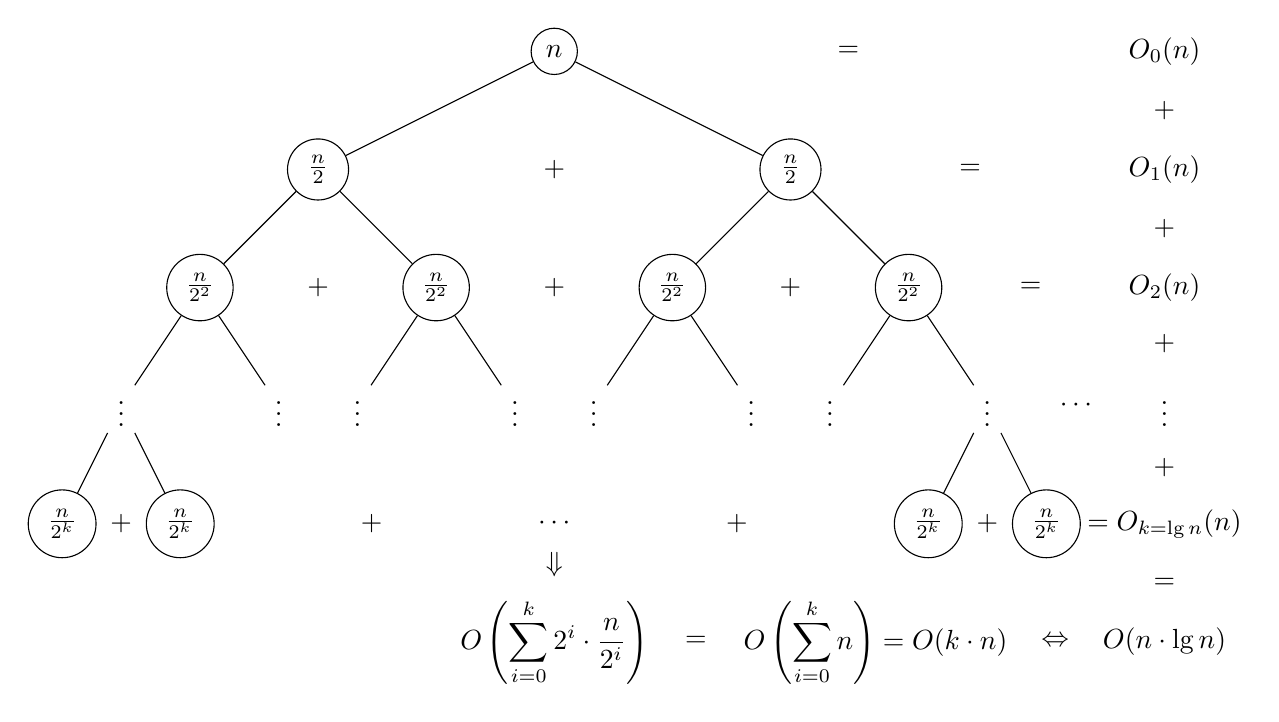
\begin{tikzpicture}[level/.style={sibling distance=60mm/#1}]
\node [circle,draw] (z){$n$}
  child {node [circle,draw] (a) {$\frac{n}{2}$}
    child {node [circle,draw] (b) {$\frac{n}{2^2}$}
      child {node {$\vdots$}
        child {node [circle,draw] (d) {$\frac{n}{2^k}$}}
        child {node [circle,draw] (e) {$\frac{n}{2^k}$}}
      }
      child {node {$\vdots$}}
    }
    child {node [circle,draw] (g) {$\frac{n}{2^2}$}
      child {node {$\vdots$}}
      child {node {$\vdots$}}
    }
  }
  child {node [circle,draw] (j) {$\frac{n}{2}$}
    child {node [circle,draw] (k) {$\frac{n}{2^2}$}
      child {node {$\vdots$}}
      child {node {$\vdots$}}
    }
  child {node [circle,draw] (l) {$\frac{n}{2^2}$}
    child {node {$\vdots$}}
    child {node (c){$\vdots$}
      child {node [circle,draw] (o) {$\frac{n}{2^k}$}}
      child {node [circle,draw] (p) {$\frac{n}{2^k}$}
          child [grow=right] {node (q) {$ = O_{k = \lg n}(n)$} edge from parent[draw=none]
            child [grow=up] {node (r) {$\vdots$} edge from parent[draw=none]
              child [grow=up] {node (s) {$O_2(n)$} edge from parent[draw=none]
                child [grow=up] {node (t) {$O_1(n)$} edge from parent[draw=none]
                  child [grow=up] {node (u) {$O_0(n)$} edge from parent[draw=none]}
                }
              }
            }
            child [grow=down] {node (v) {$O(n \cdot \lg n)$}edge from parent[draw=none]}
        }
      }
    }
  }
};
\path (a) -- (j) node [midway] {+};
\path (b) -- (g) node [midway] {+};
\path (k) -- (l) node [midway] {+};
\path (k) -- (g) node [midway] {+};
\path (d) -- (e) node [midway] {+};
\path (o) -- (p) node [midway] {+};
\path (o) -- (e) node (x) [midway] {$\cdots$}
  child [grow=down] {
    node (y) {$O\left(\displaystyle\sum_{i = 0}^k 2^i \cdot \frac{n}{2^i}\right)$}
    edge from parent[draw=none]
  };
\path (q) -- (r) node [midway] {+};
\path (s) -- (r) node [midway] {+};
\path (s) -- (t) node [midway] {+};
\path (s) -- (l) node [midway] {=};
\path (t) -- (u) node [midway] {+};
\path (z) -- (u) node [midway] {=};
\path (j) -- (t) node [midway] {=};
\path (y) -- (x) node [midway] {$\Downarrow$};
\path (v) -- (y)
  node (w) [midway] {$O\left(\displaystyle\sum_{i = 0}^k n\right) = O(k \cdot n)$};
\path (q) -- (v) node [midway] {=};
\path (e) -- (x) node [midway] {+};
\path (o) -- (x) node [midway] {+};
\path (y) -- (w) node [midway] {$=$};
\path (v) -- (w) node [midway] {$\Leftrightarrow$};
\path (r) -- (c) node [midway] {$\cdots$};
\end{tikzpicture}}
\caption{Lorem ipsum dolor sit amet}\label{img:index}
\end{figure}
%-------------------------------------------------------------------------------


%-------------------------------------------------------------------------------
% Code
%-------------------------------------------------------------------------------
\begin{lstlisting}[caption={Zbytečný kód},label=list:8-6,captionpos=b,float,abovecaptionskip=-\medskipamount,abovecaptionskip=\medskipamount,language=C]
    #include<stdio.h>
    #include<iostream>
    // A comment
    int main(void)
    {
        printf("Hello World\n");
        return 0;
    }
\end{lstlisting}

%%%%%%%%%%%%%%%%%%%%%%%%%%%%%%%%%
% alternative using package minted for source highlighting
% package minted requires execution with `-shell-escape'
% e.g., `xelatex -shell-escape ctufit-thesis.tex'
% \begin{listing}
% \begin{minted}{C}
%     #include<stdio.h>
%     #include<iostream>
%     // A comment
%     int main(void)
%     {
%         printf("Hello World\n");
%         return 0;
%     }
% \end{minted}
% \caption{Zbytečný kód}\label{list:8-6}
% \end{listing}
% %%%%%%%%%%%%%%%%%%%%%%%%%%%%%%%%%

%-------------------------------------------------------------------------------
% Table
%-------------------------------------------------------------------------------
\begin{table}\centering
	\begin{tabular}{l|l|c|c}
		Typ       & Prostředí          & \LaTeX{}ovská zkratka & \TeX{}ovská zkratka	\tabularnewline \hline
		Text      & \verb|math|        & \verb|\(...\)|        & \verb|$...$|	\tabularnewline \hline
		Displayed & \verb|displaymath| & \verb|\[...\]|        & \verb|$$...$$|	\tabularnewline
	\end{tabular}
	\caption[Příklad tabulky]{Zadávání matematiky}
	\label{tab:matematika}
\end{table}

%-------------------------------------------------------------------------------
\paragraph{Nadpis 5. úrovně}

%-------------------------------------------------------------------------------
\begin{definition}[Optional label]

\end{definition}

\begin{example}

\end{example}


\begin{theorem}

\end{theorem}

\begin{proof}

\end{proof}

\paragraph{Level 5 heading}

\begin{corollary}

\end{corollary}

\begin{proposition}

\end{proposition}

\begin{note}

\end{note}

\begin{remark}

\end{remark}

\begin{lemma}

\end{lemma}

\begin{description}
	\item[Chapter 1] I don't know
\end{description}
%-------------------------------------------------------------------------------


\appendix\appendixinit{} % do not remove these two commands

\include{text/appendix} % include `appendix.tex' from `text/' subdirectory

\backmatter{} % do not remove this command

% print out the BibLaTeX-generated bibliography list
\printbibliography{}


\chapter{Attachments}%
\label{chapter:attachments}

\todo[inline]{ Don't include other files ---
	NAC\_benchmark.ipynb,
	Visualization.ipynb,
	graphs-store/README.md,
}

\dirtree{%
	.1 thesis.pdf                           \DTcomment{thesis text in PDF}.
	%
	.1 thesis                               \DTcomment{source files of the text part}.
	.2 assets                               \DTcomment{static images and PDF attachments}.
	.3 declaration.pdf                      \DTcomment{declaration from KOS information system}.
	.2 figures                              \DTcomment{figures generated from benchmarks in PGF}.
	.2 text                                 \DTcomment{\TeX{} files of individual chapters}.
	.2 scripts														  \DTcomment{scripts for building \TeX{} files}.
	.3 rewrite\_figures.py 								  \DTcomment{updates styling in Matplotlib figures}.
	.2 ctufit-thesis.cls                    \DTcomment{FIT CTU \TeX{} template by Tomáš Nováček}.
	.2 Dockerfile                           \DTcomment{\TeX{} build image definition}.
	.2 docker-compose.yaml                  \DTcomment{Docker compose configuration for building}.
	.2 README.md                            \DTcomment{swift description of the project}.
	.2 thesis.tex                           \DTcomment{main \TeX{} document}.
	%
	.1 code                                 \DTcomment{source files of the code part}.
	.2 benchmarks                           \DTcomment{}.
	.3 precomputed                          \DTcomment{precomputed benchmark results in CSV}.
	.3 dataset.py                           \DTcomment{loads datasets from \texttt{graphs\_store}}.
	.3 generators.py                        \DTcomment{generate graphs from some graph classes}.
	.3 notebook\_utils.py                   \DTcomment{helpers for \texttt{NAC\_presentation.ipynb}}.
	.2 graphs\_store                        \DTcomment{datasets for benchmarking}.
	.3 nauty                                \DTcomment{graphs generated using Nauty}.
	.4 minimally\_rigid\_all                \DTcomment{minimally rigid graphs}.
	.5 minimally\_rigid\_\{n\}.g6           \DTcomment{graphs of vertex no \( n \)}.
	.4 generate\_minimally\_rigid\_graphs.sh\DTcomment{}.
	.3 no\_3\_nor\_4\_cycles                \DTcomment{graphs with no 3 nor 4 cycles}.
	.4 c34\_n\{n\}e\{m\}.s6                 \DTcomment{graphs with \( n \) vertices and \( m \) edges}.
	.3 random                               \DTcomment{randomly generated graphs}.
	.4 globally\_rigid                      \DTcomment{}.
	.5 globally\_rigid\_\{n\}.g6            \DTcomment{graphs of vertex no \( n \)}.
	.4 minimally\_rigid                     \DTcomment{}.
	.5 minimally\_rigid\_\{n\}.g6           \DTcomment{graphs of vertex no \( n \)}.
	.4 no\_NAC\_coloring\_graphs            \DTcomment{graphs with no NAC-coloring}.
	.5 no\_NAC\_coloring-\{n\}-TRIANGLES.g6 \DTcomment{graphs of vertex no \( n \)}.
	.5 search\_no\_NAC\_graphs.py           \DTcomment{}.
	.2 nac                                  \DTcomment{Algorithms in \Cref{chapter:nac}}.
	.3 util                                 \DTcomment{helper modules}.
	.4 \_\_init\_\_.py                      \DTcomment{}.
	.4 lazy\_product.py                     \DTcomment{lazy product of lazy iterators}.
	.4 repeatable\_iterator.py              \DTcomment{wraps lazily an iterator into a list}.
	.4 union\_find.py                       \DTcomment{\textsc{UnionFind} data structure}.
	.3 \_\_init\_\_.py                      \DTcomment{}.
	.3 algorithms.py                        \DTcomment{\Naive{}, \NaiveCycles{} and \Subgraphs{}}.
	.3 check.py                             \DTcomment{\IsNACColoring{}}.
	.3 core.py                              \DTcomment{}.
	.3 cycle\_detection.py                  \DTcomment{approaches described in \Cref{sec:small_cycles}}.
	.3 data\_type.py                        \DTcomment{}.
	.3 development.py                       \DTcomment{development helpers}.
	.3 entry.py                             \DTcomment{algorithm's API entry points}.
	.3 exception.py                         \DTcomment{}.
	.3 existence.py                         \DTcomment{\Cref{sec:polynomial_optimizations}}.
	.3 monochromatic\_classes.py            \DTcomment{\trcon{} components and monochromatic classes}.
	.3 search.py                            \DTcomment{chooses the correct algorithm}.
	.3 single.py                            \DTcomment{entry point for optimized single coloring search}.
	.3 strategies.py                        \DTcomment{approaches described in \Cref{sec:combining}}.
	.2 NAC\_playground.ipynb                \DTcomment{simple usage example}.
	.2 NAC\_presentation.ipynb              \DTcomment{benchmarking and analytics}.
	.2 pytest.ini                           \DTcomment{configuration for pytest}.
	.2 README.md                            \DTcomment{environment setup instructions}.
	.2 requirements.txt                     \DTcomment{Python dependencies with specified version}.
	.2 shell.nix                            \DTcomment{environment setup for NixOS}.
	.2 stablecut                            \DTcomment{based on \Cref{chapter:stable_cuts}}.
	.3 \_\_init\_\_.py                      \DTcomment{}.
	.3 flexible\_graphs.py                  \DTcomment{\Cref{alg:stable_cut_flexible}}.
	.3 types.py                             \DTcomment{}.
	.3 util.py                              \DTcomment{}.
	.2 test                                 \DTcomment{tests using Pytest}.
	.3 \_\_init\_\_.py                      \DTcomment{}.
	.3 test\_nac.py                         \DTcomment{tests for NAC-coloring algorithms}.
	.3 test\_stablecut.py                   \DTcomment{tests for stable cut algorithms}.
}

 % include `medium.tex' from `text/' subdirectory

\end{document}
